\documentclass{article}

\usepackage{fullpage}
\usepackage{amsmath}
\usepackage{hyperref}
\usepackage{listings}
\usepackage{graphicx}

\lstset{basicstyle=\footnotesize\ttfamily}

\title{Documentation for the \texttt{veff} package}
\author{Sam McSweeney}

\newcommand{\veff}{\texttt{veff}}
\newcommand{\parabfit}{\texttt{parabfit}}
\newcommand{\ggb}{\texttt{ggb}}

\newcommand{\x}{\texttt{x}}
\newcommand{\y}{\texttt{y}}
\newcommand{\s}{\texttt{s}}

\begin{document}

\maketitle
\tableofcontents

\section{Overview}

\veff{} is a set of programs designed for the analysis of pulsar secondary spectra.
It comprises three components: \parabfit{}, \veff{}, and \ggb{}.
\begin{itemize}
    \item \underline{\parabfit}: Fits a parabola to a secondary spectrum of the pulsar.
    \item \underline{\veff}: Analyses the relative motions of the Earth and the pulsar, projected onto the plane of the sky.
    \item \underline{\ggb}: Creates a visualisation of the Earth/pulsar system using the program Geogebra.
\end{itemize}

\section{Installation}

The \veff{} program depends on CSPICE (\url{https://naif.jpl.nasa.gov/naif/toolkit_C.html}).
Follow the directions on their website to install the C toolkit for CSPICE on your system.
Once CSPICE is installed, open the \texttt{Makefile} in the base directory where you cloned this repo and edit the \texttt{CSPICE\_DIR} variable to point to the location of your CSPICE installation.

You may also like to edit \texttt{INSTALL\_DIR} to the location of your choice.
This is where the \veff{} and \parabfit{} binaries will be copied during installation.

Finally, run \texttt{make} and \texttt{make install}.

For typeset documentation, run \texttt{make documentation}.
The documentation is found in \texttt{doc/doc.pdf}.

\section{The \parabfit{} program}

\parabfit{} takes as input a secondary spectrum of a pulsar and outputs the curvature of a fitted parabola.
The parabola fit is obtained via a generalised Hough Transform, with user-specified search parameters.

\subsection{Secondary spectrum format}

The secondary spectrum must be a text file containing three columns of numbers, here labeled \x{}, \y{}, and \s{}, respectively representing the $x$-coordinate, the $y$-coordinate, and the value at those coordinates of the secondary spectrum.
\x{} and \y{} \emph{must} be integers with the bottom-left pixel of the secondary spectrum corresponding to (\x{},\y{}) = (1,1).
The order of the lines do not matter, except that the last line must contain the top-right pixel.
(This is because the last line is used to discover how large to make the 2D array.)

\begin{lstlisting}[frame=single,title=Example secondary spectrum file with dimensions (3:4)]
1 1   0.177642
1 2  -0.243767
1 3   0.106081
1 4   0.378295
2 1   0.988884
2 2  -1.071105
2 3   0.989299
2 4  -0.075188
3 1   1.146344
3 2   0.580362
3 3  -0.465364
3 4   2.905897
\end{lstlisting}

\subsection{Command line arguments}

The basic usage of \parabfit{} is
\begin{lstlisting}
  > parabfit [OPTIONS] DATAFILE
\end{lstlisting}
\texttt{DATAFILE} is the required path to the secondary spectrum file.
The options are
\begin{description}
    \item[\texttt{--orig=X,Y}] The X,Y values corresponding to the origin of the secondary spectrum (i.e. the DC bin). X and Y are allowed to be floating point numbers, but they should be given in units corresponding to the input file. If the example secondary spectrum above were being used with the option \texttt{--orig=2,2.5}, the origin would be placed midway between the pixels containing values $-1.071105$ and $0.989299$. The default values are 0.0,0.0, which are almost certainly not what you want.
    \item[\texttt{--units=XY}] The named units corresponding to the X and Y axes of the secondary spectrum. The default values are ``\texttt{mHz}'', ``\texttt{$\mu$s}''. There is no physical meaning associated with these units---they are merely used to decorate the outputs with appropriate units.
    \item[\texttt{--res=X,Y}] The resolution of the $x$- and $y$-axes. That is, these are the widths and heights (respectively) of individual pixels in the secondary spectrum. These should be given in physical units.
    \item[\texttt{--xrange=LO,HI}] The minimum and maximum values of $x$ (in physical units) to consider. The resulting outputs (see \texttt{--out} and \texttt{--ssgpi}) will only contain data within this specified region. This is effectively a cropping operation, which takes place \emph{before} the Hough Transform is calculated. The default values are -20.0,20.0.
    \item[\texttt{--yrange=LO,HI}] Same as \texttt{--xrange}, but for the $y$-direction. Defaults are 0.0,20.0.
    \item[\texttt{--mask=X,Y}] Data points less than these distances (in physical units) from the $x$- and $y$-axes respectively are not included in the Hough Transform. This is primarily to mitigate low-axis noise in the secondary spectrum that might erroneously contribute to Hough Transform bins corresponding to parabolas with very small and very large curvatures. The mask boundaries are represented by green lines in the output plots (see \texttt{--ssgpi}). Defaults are 0.0,0.0 (equivalent to their being no masking of any data).
    \item[\texttt{--omask=OX,OY}] Similarly to \texttt{--mask}, this causes the Hough Transform to ignore certain pixels in the secondary spectrum. In this case, the ignored pixels are those within the ellipse defined by
        \[ \left(\frac{x}{\texttt{OX}}\right)^2 + \left(\frac{y}{\texttt{OY}}\right)^2= 1, \]
        centered on the origin (with $x$ and $y$ given in physical units). Like \texttt{--mask}, this is represented by a green curve in the \texttt{--ssgpi} output plot.
    \item[\texttt{--pdist=DX,DY}] This tells the Hough Transform which pixels to include for a given parabola. A pixel is included if it is both no more than a horizontal distance \texttt{DX} and no more than a vertical distance \texttt{DY} from the parabola in question, where \texttt{DX} and \texttt{DY} are to be given in physical units. Defaults are 1.0,1.0.
    \item[\texttt{--dB}] Treats the secondary spectrum values as logarithmic dB units. This makes no difference to the calculation of the Hough Transform; it merely labels the axes accordingly on the output plots (see \texttt{--ssgpi} and \texttt{--hggpi}). Default value is ``off'' (i.e. values are treated as amplitudes).
    \item[\texttt{--logspace}] Instructs the Hough Transform to interpolate the values given by \texttt{--curves} evenly on a logarithmic scale. For example, if \texttt{--curves=0.25:2.0:4}, then without \texttt{--logspace}, the Hough Transform is sampled at [0.25, 0.833, 1.417, 2.0]; with \texttt{--logspace}, at [0.25, 0.5, 1.0, 2.0]. Also, the Hough Transform plot (\texttt{--hggpi}) is given a logarithmic $x$-axis. Default is ``off''.
    \item[\texttt{--curves=START:END:N}] This defines the scope of the Hough Transform. \texttt{N} parabolic curvates are sampled between \texttt{START} and \texttt{END}. See \texttt{--logspace} for a description of how the interpolated values are calculated. Note that reducing the range while keeping \texttt{N} constant produces a finer sampling of the Hough Transform at no extra computational cost. Default values are 0.1:10.0:1000.
    \item[\texttt{--q1, --q2, --q3, --q4}] Defines which quadrants of the secondary spectrum to include in the Hough transform:
        \begin{tabular}{c|c}
            2 & 1 \\
            \hline
            3 & 4
        \end{tabular}.
        Typically, the secondary spectrum data are the amplitudes of a DFT of real values, in which case quadrants 1 and 2 are the same as quadrants 3 and 4 respectively. This option is most useful when a parabolic arc is clear on one side but diffuse on the other. Ignoring the diffuse quadrant can improve the signal-to-noise of the Hough Transform result. If no quadrants are selected, the options will default to \texttt{--q1} and \texttt{--q2}.
    \item[\texttt{--out=FILE}] The result of the Hough Transform will be written to FILE in a text format. The columns of FILE are (1) the curvature of the parabola, (2) the sum of the pixels along that parabola, and (3) the number of pixels included in the sum. This file can be plotted with the gnuplot script generated by the \texttt{--hggpi} option. If \texttt{--out} is not supplied, no output will be written, and attempting to supply \texttt{--hggpi} will result in an error.
    \item[\texttt{--hggpi=FILE}] A gnuplot script for viewing the file set by the \texttt{--out} option will be written to FILE. If the \texttt{--out} option has not been supplied, this option will result in an error.
    \item[\texttt{--crop=FILE}] The cropped secondary spectrum (see \texttt{--xrange} and \texttt{--yrange}) will be written to FILE in a binary format. This file can be plotted with the gnuplot script generated by the \texttt{--ssgpi} option. If \texttt{--crop} is not supplied, no output will be written, and attempting to supply \texttt{--ssgpi} will result in an error.
    \item[\texttt{--ssgpi=FILE}] A gnuplot script for viewing the file set by the \texttt{--crop} option will be written to FILE. If the \texttt{--crop} option has not been supplied, this option will result in an error.
    \item[\texttt{--cbrange=MIN,MAX}] Set the dynamic range of the output plot (see \texttt{--ssgpi}). If not supplied, Gnuplot will detect the range automatically (using the minimum and maximum values in the cropped secondary spectrum).
    \item[\texttt{-h, --help}] Display online help.
\end{description}

\subsection{Working example}

In the \texttt{test\_example} subdirectory, you will find an example secondary spectrum, \texttt{ss.out}.
The \parabfit{} program can be run on it by running the command \texttt{make parabfit} (within the \texttt{test\_example} directory).
This generates a number of outputs.
First and foremost, the curvature of the best parabolic fit is written to the terminal. In this case, the answer should be $0.8063\,\mu$s/mHz$^2$.
Secondly, a number of output files should appear in the same directory: \texttt{cropped.ss}, \texttt{cropped.ss.gpi}, \texttt{ss\_Q12.hg.txt}, and \texttt{ss\_Q12.hg.gpi}, corresponding to the options \texttt{--crop}, \texttt{--ssgpi}, \texttt{--out}, and \texttt{--hggpi} respectively.
All but the first are human-readable text files.
See the following section for how to view the Gnuplot plots.

\subsection{Viewing \parabfit{} output plots}

The files generated by the \texttt{--ssgpi} and \texttt{--hggpi} options are Gnuplot scripts.
To view the plots, open a Gnuplot terminal and write
\begin{lstlisting}
  gnuplot> load 'cropped.ss.gpi'
\end{lstlisting}
or
\begin{lstlisting}
  gnuplot> load 'ss_Q12.hg.gpi'
\end{lstlisting}
for the secondary spectrum and Hough transform plots, respectively (the file names should of course be changed to the chosen file name arguments supplied with the \texttt{--ssgpi} and \texttt{--hggpi} options).
If the plots need to be tweaked in any way, one can do so by directly manipulating the Gnuplot scripts.

To save the plots as images, preface the plot scripts with the appropriate \texttt{set terminal} and \texttt{set output} commands (see Gnuplot documentation for details).

\begin{figure}[!ht]
    \centering
    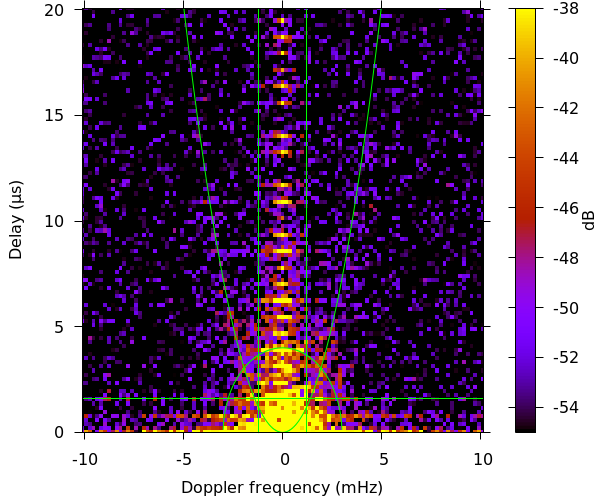
\includegraphics[scale=0.3]{example_ss.png}
    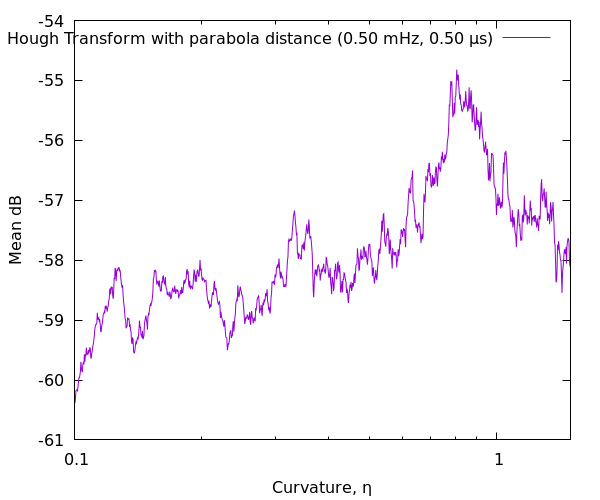
\includegraphics[scale=0.3]{example_hg.png}
\end{figure}

\section{The \veff{} program}

\end{document}
